%!TEX root = thesis.tex"`

\chapter{\Gls{pipeline} обучения}
\begin{figure}[h]
    \centering
    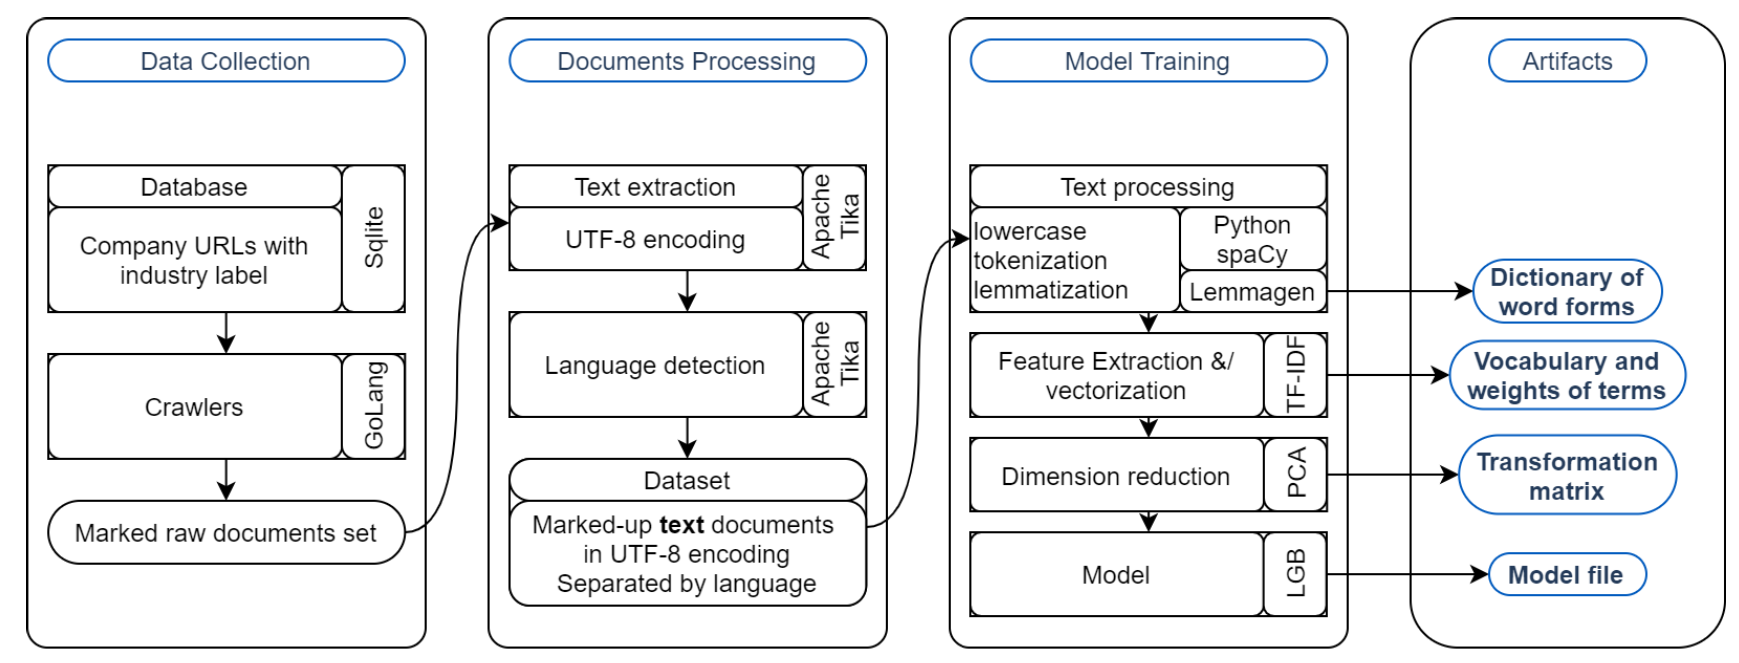
\includegraphics[width=\linewidth]{pipeline}
    \caption{Схематичное изображение процесса обучения}
    \label{fig:pipeline}
\end{figure}

В этой главе подробно описан процесс обучения, используемый в работе.
Он состоит из трех стадий:
\begin{enumerate}
    \item Сбор данных (data collection), см. \ref{sec:data-mining}.
    \item Обработка (processing) собранных документов, см. \ref{sec:preprocessing}.
    \item Обучение модели и сохранение артефактов, см. \ref{sec:training}.
\end{enumerate}
Каждая из этих стадий будет раскрыта подробнее в дальнейших секциях.

\section{Структура данных}
\subsection{Сырые данных}
В настоящей работе в качестве входных данных выступают документы, выгруженные из открытых источников в сети Интернет.
Данные представляют из себя веб-страницы, сохраненные локально в разнообразных форматах (HTML, PDF, .doc и другие).
Сопутствующий мультимедийный контент (видеозаписи, аудизаписи, картинки и т.п.) не сохраняется и не учитвается в модели.
Любой язык разметки, метаинформация, скрипты и таблицы стилей (в случае HTML) сохраняются в сырых документах <<как есть>>.

Все документы, участвующие в процессе, делятся на категории.
Категории заранее фиксированы и размечаются вручную.
Ниже приведен их список:
\label{categories}
\begin{itemize}
    \item Sales, Marketing and PR
    \item HR
    \item Finance and Banking
    \item IT, IT research and Development
    \item Manufacturing
    \item Medical and Paramedical
    \item Business and Corporate
    \item Legal
    \item Others
\end{itemize}

Разметка сырых данных фиксируется на уровне веб-сайта, т.е. \textbf{все} документы одного веб-сайта относятся к одинаковой категории.
Такой способ разметки является приближенным, поскольку один и тот же веб-сайт может содержать документы, относящиеся к различным тематикам (к примеру, медицинский сайт может содержать помимо мед.документов образцы договоров об оказании платных услуг).
\subsection{Данные для обучения}
Модель классификатора реализована на очищенных и нормализованных документах.
Данные для обучения представляют из себя набор файлов (по одному на каждую категорию из \ref{categories}), каждый из которых содержит множество документов.

Каждый документ в таком файле представляет из себя одну строку, которая заполнена словами в свой начальной форме, разделенными пробелом.
В таком формате данные предстают в человекочитаемом виде и то же время могут быть легко обрабтаны компьютером.

\section{Получение сырых данных}
\label{sec:data-mining}
\subsection{Общее описание \gls{crawler}}
\begin{wrapfigure}{r}{7cm}
    \centering
    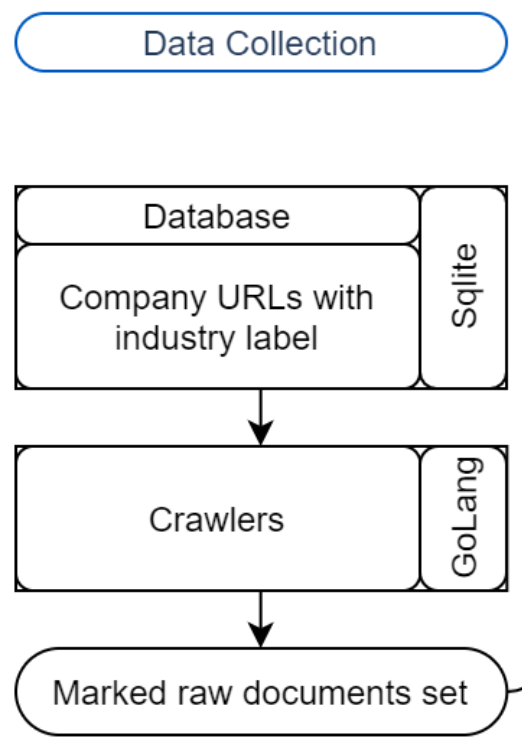
\includegraphics[width=\linewidth]{crawlers-pipeline}
    \caption{Архитектура \gls{crawler}}
    \label{fig:crawler-pipeline}
\end{wrapfigure}
Для получения документов была разработана программа для выгрузки веб-страниц (\gls{crawler}).
Для достижения большей производительности \gls{crawler} был написан на языке \gls{golang}, сочетающим высокую скорость работы и относительную простоту написания кода.

Схематично архитектура краулера показана на рис. \ref{fig:crawler-pipeline}.
На каждую поддерживаемую локализацию заводится своя база данных, содержащая ссылки сайтов, сгруппированные по категории.
Категории сайта записываются в базу данных вместе с множеством URL-адресов - пример этого изображен на рис. \ref{fig:crawler-db-head}.
Такая БД содержит немного данных, поэтому для простоты интеграции с \gls{golang} в качестве \acrshort{dbms} используется \gls{sqlite}.

\begin{figure}[h]
    \centering
    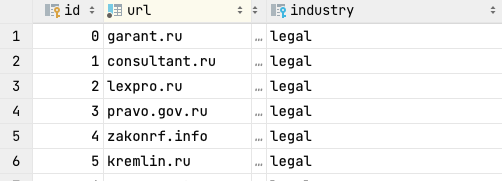
\includegraphics[width=0.8\linewidth]{crawler-db-head}
    \caption{Пример данных из БД краулера}
    \label{fig:crawler-db-head}
\end{figure}
Файл с заполненной базой данных поступает на вход программе \gls{crawler} (второй большой прямоугольник на \ref{fig:crawler-pipeline}), который запускет обход в глубину каждого URL-адреса.
В каждом выгруженном веб-сайте ищутся все возможные гиперссылки на другие страницы, и эти гиперссылки добавляются в очередь выгрузки.
Процесс продоложается до тех пор, пока вся очередь выгрузки для данного сайта не будет исчерпана, либо не будет достигнут лимит на количество загружаемых документов с одной страницы (\crawlerPageLimit).
\subsection{Типы используемых \gls{crawler}}
Существует несколько типов краулеров и подходов к их реализации \cite{cite:crawler-review}.
Помимо этого на стороне сайта возможно применение методов защиты от автоматической выгрузки \cite{cite:crawler-protection}.
Это, с одной стороны, создает некоторую вариативность, а с другой стороны -- обязывает иметь запасные варианты реализации сбора данных с веб-страниц.
С учетом данных факторов в настоящей работе используется три типа \gls{crawler}: \textit{google crawler}, \textit{colly crawler} \cite{cite:colly} и \textit{common index crawler} \cite{cite:common-crawl}.

Google \gls{crawler} напрямую запрашивает все документы с сайта через веб-поисковик \url{https://google.com}.
Этот метод весьма эффективен, т.к. полагается на собираемый Google индекс сайтов, но в то же время очень ограничен, т.к. \url{google.com} достаточно быстро начинает запрашивать CAPTCHA при запросе.
Обойти проверку CAPTCHA возможно несколькими способами, описанными, к примеру, в \cite{cite:captcha-bypass-1} и \cite{cite:captcha-bypass-2}.
Однако все эти способы требуют большие вычислительные мощности, что не удовлетворяло требованию о быстрой работе краулера.
Поэтому были разработы другие краулеры.

Common Index \gls{crawler} запрашивает копию страницы из интернет-архива \href{https://commoncrawl.org/}{Common Crawl}.
Это -- самый безотказный способ, т.к. веб-архив не требует ввода CAPTCHA и имеет нестрогие ограничения на количество запросов.
Тем не менее, архив может содержать не все страницы и скорость загрузки может быть ограничена из-за технических особенностей платформы.

Colly \gls{crawler} \cite{cite:colly} является самым продвинутым из описанных краулеров.
В то время как остальные \gls{crawler} полагаются на сторонние ресурсы, colly самостоятельно проходит по всем сайтам, выискивая все возможные гиперссылки на другие документы и проходя по ним в следующей итерации.
Такой алгоритм приводит к тому, что выгружаются практически все документы с сайта (кроме тех, что защищены авторизацией или проверками на ботов).
К сожалению, на больших сайтах алгоритм может достаточно долго блуждать по гиперссылкам.
Более того, нет никакой гарантии, что полученный граф обхода не содержит циклов, поэтому colly crawler может потенциально уйти в вечный цикл.
Для защиты от указанных проблем в данном \gls{crawler} выставлен лимит на время выполнения (\collyTimeLimit) и суммарный размер выгружаемых документов (\collySizeLimit).

Использование всех трех краулеров показало хорошие результаты -- по каждому языку было выгружено около \datasetSize сырых документов, что составило порядка \datasetDocs документов.

\section{Преобразование сырых данных в данные для модели}
\label{sec:preprocessing}
Как уже было сказано в главе \ref{chapter-1}, работа с текстом зачастую подразумевает его преобразование в вектора.
В данной работе указанный процесс, осуществляемый над сырыми данными, происходит в три стадии:
\begin{enumerate}
    \item Очистка текста от разметки и служебной информации.
    \item Выделение \textit{токенов} -- отдельных единиц языка в начальной форме.
    \item Непосредственное преобразование токенов каждого текста в вектора посредством \acrshort{tf-idf}.
\end{enumerate}
Остановимся кратко на каждом шаге.
\subsection{Очистка текста}
Для очистки текста от разметки и служебной информации используется программа \gls{apache} \gls{tika}.
Данная программа была выбрана по нескольким причинами:
\begin{enumerate}
    \item Скорость.
        \Gls{tika} быстро обрабатывает документы -- упомянутые 200 тысяч документов обрабатываются за 10 минут, что является хорошей скоростью по сравнению с остальными стадиями всего \gls{pipeline}.
    \item Зрелость продукта.
        \Gls{tika} разработывется фондом \Gls{apache}, что дает некоторые гарантии по стабильности продукта.
        Проект развивается с 2007 года и в настоящее время находится в зрелом состоянии.
    \item Поддержка большого числа форматов.
        На \href{https://tika.apache.org/1.10/formats.html}{официальной странице} используемой в проекте версии \gls{tika} заявляется поддержка более 20 форматов.
\end{enumerate}
С примерами данных после работы \Gls{tika} можно ознакомиться в листинге \ref{listing:tika-example}.
% TODO: (ruapyyj) рассказ про тику <- Thu Apr 21 13:26:19 2022
\subsection{Выделение токенов}
Для выделения токенов и приведения слов к нормальной форме (лемматизация, \gls{lemmatization}) существует несколько подходов \cite{cite:lemmatization-review}.
В данной работе рассматривалась работа на \gls{spacy} \cite{cite:spacy} и на \gls{nltk} \cite{cite:nltk}.

\gls{spacy} предоставляет богатый набор возможностей для обработки текста и построении на его основе комплексных \acrshort{ml} моделей.
В то же время данных фреймворк достаточно требователен к ресурсам, и даже частичное использование его языковых возможностей сопряжено с большими вычистительными затратами.
Несмотря на проведенные оптмизации и настройку \gls{pipeline} обработки текста, \gls{spacy} показал низкую скорость работы и стал лимитирующей стадией во всем \gls{pipeline} обучения.
Так, обработка одной локализации размером \datasetSize занимала у \gls{spacy} порядка трех дней, что сильно замедляло скорость разработки и проведения экспериментов.

Для расширения поддержки нескольких локализаций это стало недопустимым, и поэтому были проведены работы по поиску более производительных альтернатив, способных предоставить схожее качество лемматизации документов.
В качестве достойной альтернативы был выбран фреймворк \gls{nltk}, который смог полностью удовлетворить потребности по лемматизации.
Во-первых, \gls{nltk} имел встроенные алгоритмы \gls{lemmatization}, которые выдавали данные, схожие с выходными данными \gls{spacy}.
Во-вторых, скорость работы \gls{nltk} была на порядок выше скорости работы \gls{spacy}.
Уже упомянутый набор данных размером \datasetSize обрабатывался на \gls{nltk} за 20 минут, что было сопоставимо с остальными стадиями всего \gls{pipeline} обучения.

По итогу сравнения двух фреймворков был выбран \gls{nltk} в качестве токенизатора.
С примерам данных, получаемых в ходе его работы, можно ознакомиться в листинге \ref{listing:tokenizer-example}.
\subsection{Преобразование в \acrshort{tf-idf}}
\label{par:tf-idf}
Для преобразования полученных после токенизации слов в векторы использется мера \acrfull{tf-idf} -- один из самых простых и первых способов векторного представления текста, который позволяет также изучать значимость слов \cite{cite:tf-idf-interpretation}.
Само преобразование просто: для каждого слова $t$ в документе $d$ из коллекции $D$ вычисляется мера:
\begin{equation}
    \label{eq:tf-idf}
    \text{tf-idf} (t, d, D) = \text{tf} (t, d) \cdot \text{idf} (t, D),
\end{equation}
которая состоит из двух компонент -- \acrfull{tf} и \acrfull{idf}.
\acrshort{tf} есть
\begin{equation}
    \label{eq:tf}
    \text{tf} (t, d) = \cfrac{n_t}{\sum_k n_k},
\end{equation}
где $n_t$ -- число вхождений слова $t$ в документ, а $\sum_k n_k$ представляет из себя общее число слов в данном документе.

\acrshort{idf} определяется как
\begin{equation}
    \label{eq:idf}
    \text{idf} (t, D) = \log \cfrac{|D|}{|\{d_i \in D | t \in d_i\}|},
\end{equation}
где $|D|$ -- общее число документов в коллекции, а знаменатель равен числу документов из коллекции $D$, в которых встречается $t$ (т.е. $n_t \neq 0$).

Данная метрика для слова из документа имеет интуитивную интерпретацию.
Ее \acrshort{tf} часть увеличивается тогда, когда слово чаще встречается в документе, но с другой стороны, слово должно встречаться часто именно в одном документе (согласно \eqref{eq:idf}) -- это не дает частым и не несущим смысла словами (таким как артикли) набирать большое значение \acrshort{tf-idf}.
Если слово встречается во всех документах, то его значимость в смысле \acrshort{tf-idf} уменьшается за счет уменьшения второго множителя в \eqref{eq:tf-idf}.

В настоящей работе используется реализация \acrshort{tf-idf} из библиотеки \gls{scikit-learn} \cite{cite:scikit-learn}.
\section{Модель \acrshort{ml} и ее обучение}
\label{sec:training}
Преобразованные и очищенные данные поступают классификатору, непосредственно решающему поставленную задачу \acrlong{mcc}.
В данной работе в качестве алгоритма классификации рассматривался градиентный бустинг над случайными деревьями, подробно описанный в \cite{cite:xgboost}.
Данная модель базируется на следующих принципах:
\begin{enumerate}
    \item Строится множество деревьев, из которого первое дерево строится по случайной подвыборке.
    \item На каждом этапе построения дерева решение о ветвлении принимается по случайному подмножеству признаков (метод случайных подпространств).
    \item Прогноз вероятности класса $k$ определяется как доля деревьев, проголосовавших за класс $k$.
    \item Каждое следующее дерево из леса обучается не на таргете $y$, а на ошибке предыдущего классификатора и градиенте этой ошибки (gradient boosting).
\end{enumerate}
Градиентый бустинг над случайными лесами -- очень популярный алгоритм в сфере \acrshort{ml}, его часто используют в качестве базового решения задачи.

Как уже было сказано в \ref{par:tf-idf}, в настоящей работе используется \acrshort{tf-idf}, который выдает вектор с количеством компонент, равным числу уникальных слов в наборе документов.
При используемых в работе данных это число может оказаться велико даже для случайных лесов, что может негативно сказаться затрачиваемом для обучения времени.
Поэтому перед обучением на векторе \acrshort{tf-idf} проводится уменьшение размерности методом \gls{pca}.
Кратко остановимся на сущности этого метода.

Интуитивно \gls{pca} может быть представлен как аппроксимация данных неким эллипсоидом.
Оси такого эллипсоида, обладающие наибольшей длиной, будут соответствовать наибольшей дисперсии.
Оставляя только первые $L < N$ осей, можно добиться снижения размерности.
$L$ будет подбираться так, чтобы доля объясненной дисперсии оставалась в допустимых рамках.
Задача \gls{pca} сводится к задаче о сингулярном разложении матрицы данных.
Задача о сингулярном разложении достаточно хорошо изучена, подробнее о ней можно почитать в \cite{cite:svd-1}, \cite{cite:svd-2}.
% TODO: (ruapyyj) мб побольше описать SVD и PCA? Вернись сюда, если текста не хватит <- Tue Apr 26 22:40:31 2022

В данной работе используется реализация \gls{pca} из библиотеки \gls{scikit-learn} с небольшой модификацией: вместо явного задания количества компонент $L$ выставляется порог на долю объясненной дисперсии, и количесто компонент выбирается так, чтобы выставленный порог был преодолен.
Такая реализация удобна при работе с несколькими локализациями, поскольку в общем случае для каждой отдельной локализации может потребоваться свое количество компонент.

Таким образом, модель обучается на векторизованных данных усеченной размерности в соответствии с замечаниями, упомянутыми выше.
По окончании описание леса, словарь \acrshort{tf-idf} и веса \gls{pca} выгружается, сохраняются в файл, версионируются (см. \ref{sec:dvc}) и отправляются в облачное хранилище (см. \ref{sec:gcloud}).
% TODO: (ruapyyj) здесь бы неплохо ссылку на то, сколько компонент в какой модели <- Tue Apr 26 22:40:02 2022
